\section{Introduction}
\label{ref:intro}

This note presents a search for the production of supersymmetric (SUSY) stop quark pairs in events with a 
single isolated lepton, several jets, missing transverse energy, and large transverse mass. We use the full 
2011 data sample, corresponding to an integrated luminosity of \lumi. 
This search is of theoretical interest because of the critical role played 
by the stop quark in solving the hierarchy problem in SUSY models. This solution requires that the stop quark 
be light, less than a few hundred GeV and hence within reach for direct pair production. We focus on two decay modes 
$\tilde{t}\rightarrow t\chi^0_1$ and $\tilde{t}\rightarrow b \chi^+_1$  which are expected
to have large branching fractions if they are kinematically accessible, leading to:

\begin{itemize}
\item $pp\rightarrow\tilde{t}\bar{\tilde{t}}\rightarrow t\bar{t}\chi^0_1\chi^0_1$, and
\item $pp\rightarrow\tilde{t}\bar{\tilde{t}}\rightarrow b\bar{b}\chi^+_1\chi^-_1 \rightarrow b\bar{b}W^+W^-\chi^0_1\chi^0_1$.
\end{itemize}

Both of these signatures contain high transverse momentum (\pt) jets including two b-jets, and missing transverse 
energy (\MET) due to the invisible $\chi^0_1$ lightest SUSY particles (LSP's). In addition, the presence of
two W bosons leads to a large branching fraction to the single lepton final state. Hence we require the presence
of exactly one isolated, high \pt electron or muon, which provides significant suppression of several backgrounds
that are present in the all-hadronic channel. The largest backgrounds for this signature are semi-leptonic \ttbar\
and \wjets. These backgrounds contain a single leptonically-decaying W boson, and the transverse mass (\mt)
of the lepton-neutrino system has a kinematic endpoint requiring \mt $<$ $M_W$. For signal stop quark events,
the presence additional LSP's in the final states allows the \mt to exceed $M_W$. Hence we search for an excess
of events with large \mt. The dominant background in this kinematic region is dilepton \ttbar\ where one of the
leptons is not identified, since the presence of two neutrinos from leptonically-decaying W bosons allows the 
\mt\ to exceed $M_W$. Backgrounds are estimated from Monte Carlo (MC) simulation, with careful validation 
and determination of scale factors and corresponding uncertainties based on data control samples.

The expected stop quark pair production cross section (see Fig.~\ref{fig:stopxsec}) varies between O(10) pb
for $m_{\tilde{t}}=200$~GeV and O(0.01) pb for $m_{\tilde{t}}=500$~GeV. The critical challenge of this analysis
is due to the fact that for light stop quarks with a mass close to the top quark, the production cross section is
large but the kinematic distributions, in particular \mt, are very similar to SM \ttbar\ production, such that it becomes very
difficult to distinguish the signal and background. For large stop quark mass the kinematic distributions differ
from those in SM \ttbar\ production, but the cross section decreases rapidly, reducing the signal-to-background
ratio.

\begin{figure}[hbt]
  \begin{center}
	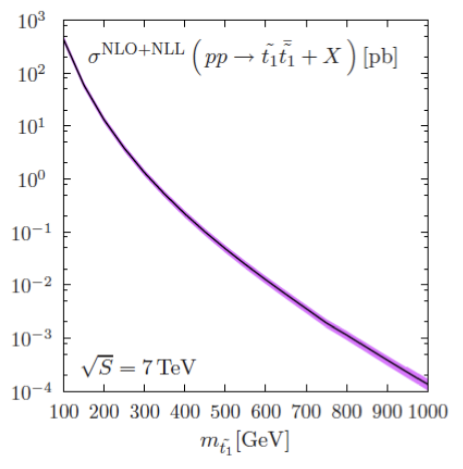
\includegraphics[width=0.4\linewidth]{plots/stop.pdf}
	\caption{
	  \label{fig:stopxsec}\protect 
          The stop quark pair production cross section in pb, as a function of the stop quark mass.}
  \end{center}
\end{figure}

